% ============================================================================
%  Rapport -- qaoa-ml-optimizer
%  Compilation (depuis docs/) : pdflatex rapport.tex (deux fois)
%  Tableaux et figures : python experiments/run_study.py  ->  results/study/
% ============================================================================
\documentclass[11pt,a4paper]{article}

\usepackage[utf8]{inputenc}
\usepackage[T1]{fontenc}
\usepackage[french]{babel}
\usepackage{lmodern}
\usepackage{microtype}
\usepackage[margin=2.5cm]{geometry}
\usepackage{amsmath,amssymb}
\usepackage{booktabs}
\usepackage{graphicx}
\usepackage{xcolor}
\usepackage{tikz}
\usetikzlibrary{babel}
\usepackage{quantikz}
\usepackage{caption}
\usepackage[hidelinks]{hyperref}

\captionsetup{font=small,labelfont=bf}
\graphicspath{{../results/study/}}
\newcommand{\etude}{../results/study}
\newcommand{\inclure}[2]{\IfFileExists{\etude/#1}{#2}{\textcolor{orange!80!black}{\textbf{À générer :}
  \texttt{python experiments/run\_study.py}}}}

\title{\textbf{Apprendre à initialiser le QAOA}\\[0.3em]
\large Prédire les angles d'un algorithme quantique d'optimisation\\ à partir de la structure du problème\\[0.3em]
\normalsize Projet 2 -- Série « IA et informatique quantique »}
\author{Deo Gratias Loutou\\ Master 1 Informatique et Mobilité -- Université de Haute-Alsace}
\date{\today}

\begin{document}
\maketitle

\begin{abstract}
Le QAOA (\emph{Quantum Approximate Optimization Algorithm}) résout des problèmes d'optimisation
combinatoire à l'aide d'un circuit quantique dont $2p$ angles sont réglés par un optimiseur classique.
Sur matériel réel, chaque évaluation du circuit est coûteuse et bruitée : le point de départ de
l'optimisation est donc déterminant. Nous entraînons des modèles d'apprentissage à prédire les angles
optimaux pour le problème MaxCut à partir de douze caractéristiques du graphe. Sur 50 graphes de test
jamais vus et pour une profondeur $p=3$, les angles prédits par un modèle des $k$ plus proches voisins
atteignent 99\,\% de l'optimum \emph{sans aucune optimisation}, et l'optimisation qui suit demande
44\,\% d'évaluations en moins qu'une initialisation heuristique en rampe et 4,5 fois moins qu'une
initialisation aléatoire. Cinq graphes d'entraînement suffisent à dépasser la simple moyenne des angles
connus, et le modèle généralise à des graphes plus grands que ceux vus à l'entraînement. Nous
rappelons enfin que, sur ces petites instances, une recherche locale classique trouve la solution
exacte en moins d'une milliseconde.
\end{abstract}

\tableofcontents
\newpage

% ----------------------------------------------------------------------------
\section{Introduction}

L'optimisation combinatoire -- planification, tournées, placement, conception de circuits -- est l'un des
domaines d'application les plus attendus de l'informatique quantique. Le QAOA, proposé par Farhi,
Goldstone et Gutmann~\cite{farhi2014}, en est l'algorithme de référence pour les machines actuelles :
il n'exige qu'un circuit de faible profondeur, complété par une boucle d'optimisation classique.

Cette boucle est le point faible de l'approche. Chaque évaluation de la fonction objectif demande
d'exécuter le circuit des centaines de fois pour estimer une moyenne, et le paysage à optimiser
comporte de nombreux optima locaux. Une bonne initialisation réduit à la fois le coût et le risque
d'échec. Or il a été observé que les angles optimaux varient peu d'une instance à l'autre
(\emph{concentration des paramètres}~\cite{brandao2018,zhou2020}), ce qui suggère qu'ils peuvent être
\emph{appris}~\cite{khairy2020}.

\paragraph{Question.} Un modèle d'apprentissage entraîné sur de petits graphes déjà résolus peut-il
proposer de meilleurs angles de départ que les heuristiques existantes, et de combien réduit-il le
nombre d'évaluations du circuit ?

% ----------------------------------------------------------------------------
\section{Le problème MaxCut}

Soit un graphe $G=(V,E)$ à $n$ sommets. Une partition est un vecteur $z \in \{0,1\}^n$ ; sa coupe est
\begin{equation}
  C(z) = \sum_{(i,j)\in E} \mathbb{1}[z_i \neq z_j].
\end{equation}
MaxCut consiste à trouver $C_{\max} = \max_z C(z)$. Le problème est NP-difficile ; l'algorithme de
Goemans et Williamson garantit un ratio de $0{,}878$ en temps polynomial~\cite{goemans1995}. Pour les
graphes étudiés ici ($n \le 12$), l'énumération des $2^n$ partitions donne la solution exacte.

% ----------------------------------------------------------------------------
\section{L'algorithme QAOA}

\subsection{Le circuit}
Chaque partition est encodée dans un état de base $\ket{z}$ de $n$ qubits. Le QAOA de profondeur $p$
prépare
\begin{equation}
  \ket{\boldsymbol\gamma,\boldsymbol\beta} =
  U_M(\beta_p)\,U_C(\gamma_p)\cdots U_M(\beta_1)\,U_C(\gamma_1)\,\ket{+}^{\otimes n},
\end{equation}
où $U_C(\gamma)=e^{-i\gamma H_C}$ applique à chaque $\ket{z}$ une phase proportionnelle à $C(z)$, et
$U_M(\beta)=e^{-i\beta\sum_k X_k}$ (des rotations $R_X(2\beta)$) fait interférer les partitions.
Le coût s'implémente avec une porte $R_{ZZ}$ par arête (figure~\ref{fig:circuit}). Un optimiseur
classique maximise la coupe moyenne $F(\boldsymbol\gamma,\boldsymbol\beta)=\langle C\rangle$ ; la
qualité d'une solution se mesure par le \emph{ratio d'approximation} $r = F/C_{\max}$.

\begin{figure}[h]
\centering
\begin{quantikz}[column sep=0.3cm]
\lstick{$\ket{0}$} & \gate{H} & \gate[2]{R_{ZZ}(\gamma)} & \gate[3, style={dashed}]{\cdots} & \gate{R_X(2\beta)} & \meter{} \\
\lstick{$\ket{0}$} & \gate{H} &                          &                                   & \gate{R_X(2\beta)} & \meter{} \\
\lstick{$\ket{0}$} & \gate{H} &                          &                                   & \gate{R_X(2\beta)} & \meter{}
\end{quantikz}
\caption{Une couche du QAOA ($p=1$) : préparation de $\ket{+}^{\otimes n}$, une porte $R_{ZZ}(\gamma)$
par arête, puis le mélangeur.}
\label{fig:circuit}
\end{figure}

\subsection{Simulation}
Le circuit est écrit avec PennyLane~\cite{pennylane}. Pour générer des milliers d'optimisations, nous
utilisons en plus un simulateur spécialisé : $U_C$ étant diagonal, il se réduit à une multiplication
terme à terme par $e^{i\gamma C(z)}$, et $U_M$ à $n$ rotations appliquées par permutation d'axes. Ce
simulateur est environ 50 fois plus rapide (0,2\,ms contre 13\,ms par évaluation à 10 qubits) et ses
résultats coïncident avec ceux de PennyLane à $10^{-8}$ près, ce que vérifient les tests automatiques.

\subsection{Optimisation et symétries}
Les angles sont optimisés par L-BFGS-B avec gradients par différences finies ; le nombre
d'évaluations rapporté inclut celles des gradients. Pour MaxCut non pondéré, $F$ est invariante par
$\gamma \to \gamma+2\pi$, $\beta \to \beta + \pi/2$ et $(\boldsymbol\gamma,\boldsymbol\beta) \to
(-\boldsymbol\gamma,-\boldsymbol\beta)$. Nous ramenons tous les angles dans une zone de référence
avant l'apprentissage : sans cette \emph{canonisation}, deux solutions équivalentes auraient des
coordonnées éloignées et brouilleraient la régression.

\paragraph{Une erreur instructive.} La convention de PennyLane ($H_C = -C$) inverse le signe
de $\gamma$ par rapport à la littérature. Notre première rampe linéaire, recopiée avec
$\beta>0$, donnait un ratio initial de $0{,}37$, \emph{pire que le hasard}. Corriger le signe l'a porté
à $0{,}80$ et a changé la conclusion de l'étude : vérifier les conventions est indispensable.

% ----------------------------------------------------------------------------
\section{Stratégies d'initialisation}

\begin{description}
  \item[Aléatoire.] $\gamma_k \sim \mathcal{U}[0,\pi]$, $\beta_k \sim \mathcal{U}[0,\pi/2]$.
  \item[Rampe linéaire.] $\gamma_k = \Delta\, t_k$, $\beta_k = -\Delta(1-t_k)$ avec
        $t_k=(k-\frac12)/p$ et $\Delta=0{,}75$ : discrétisation d'une évolution adiabatique~\cite{zhou2020}.
  \item[Moyenne.] Moyenne des angles optimaux des graphes d'entraînement : exploite la
        concentration des paramètres sans regarder le graphe. C'est la référence à battre.
  \item[Modèles appris.] Régression des $2p$ angles à partir de 12 caractéristiques : nombre de
        sommets et d'arêtes, densité, moyenne, écart-type, minimum et maximum des degrés,
        coefficient de regroupement, triangles par sommet, plus grande valeur propre et valeur de
        Fiedler du laplacien, bipartition. Trois régresseurs : $k$ plus proches voisins ($k=5$),
        forêt aléatoire (300 arbres) et perceptron multicouche ($64\times64$).
\end{description}

% ----------------------------------------------------------------------------
\section{Protocole expérimental}

\begin{itemize}
  \item \textbf{Graphes} : moitié Erdős--Rényi (probabilité d'arête entre $0{,}25$ et $0{,}75$),
        moitié réguliers de degré 3 ou 4 ; 6 à 10 sommets.
  \item \textbf{Étiquettes} : pour chaque graphe, meilleur résultat entre un départ en rampe et
        trois départs aléatoires, puis canonisation.
  \item \textbf{Données} : 200 graphes d'entraînement, 50 graphes de test générés avec une autre graine.
  \item \textbf{Métriques} : ratio d'approximation des angles proposés \emph{avant} optimisation,
        ratio final, nombre d'évaluations du circuit jusqu'à convergence, et taux de succès (ratio
        final à moins de $10^{-3}$ du meilleur connu).
  \item \textbf{Expériences} : (A) profondeurs $p = 1, 2, 3$ ; (B) courbe d'apprentissage de 5 à
        200 graphes ($p=2$) ; (C) généralisation à 30 graphes de 12 sommets ($p=2$).
\end{itemize}

% ----------------------------------------------------------------------------
\section{Résultats}

\subsection{Qualité de l'initialisation et coût}

\begin{table}[h]
\centering
\small
\inclure{table_depth.tex}{\input{\etude/table_depth.tex}}
\caption{Ratio d'approximation des angles proposés, avant toute optimisation, et nombre moyen
d'évaluations du circuit jusqu'à convergence (50 graphes de test). En gras : meilleure valeur par colonne.}
\label{tab:depth}
\end{table}

Le tableau~\ref{tab:depth} et la figure~\ref{fig:depth} montrent une hiérarchie stable pour les trois
profondeurs. Le départ aléatoire ne fait pas mieux que la superposition uniforme (angles nuls, ratio
moyen de $0{,}63$) et demande de loin le plus d'évaluations. La rampe est une heuristique solide. La moyenne des angles appris fait mieux
encore, ce qui confirme la concentration des paramètres. Les modèles $k$ plus proches voisins et forêt
aléatoire dominent : à $p=3$, ils atteignent $0{,}92$, soit 99\,\% du ratio optimal ($0{,}928$),
et le $k$-NN converge en 70 évaluations contre 126 pour la rampe et 319 pour le hasard.
Le réseau de neurones, avec 200 exemples seulement, ne fait pas mieux que la moyenne.

\begin{figure}[h]
\centering
\inclure{fig_depth.pdf}{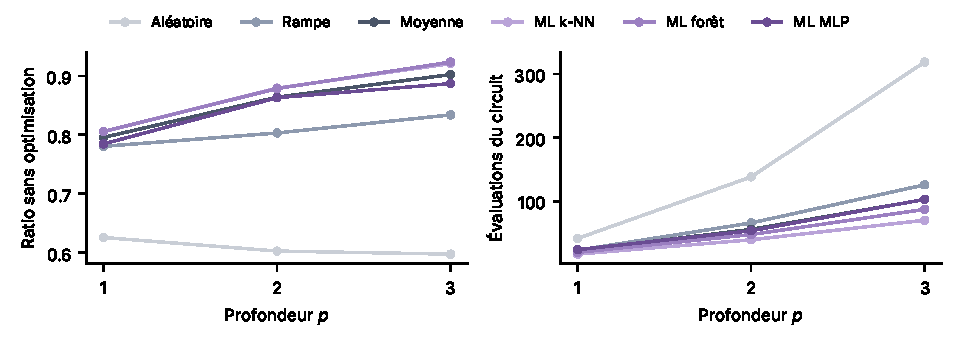
\includegraphics[width=\linewidth]{fig_depth.pdf}}
\caption{Effet de la profondeur $p$ : ratio sans optimisation (gauche) et évaluations du circuit (droite).}
\label{fig:depth}
\end{figure}

\begin{table}[h]
\centering
\small
\inclure{table_final.tex}{\input{\etude/table_final.tex}}
\caption{Ratio final après optimisation et, entre parenthèses, taux de succès (meilleur optimum connu atteint).}
\label{tab:final}
\end{table}

Après optimisation (tableau~\ref{tab:final}), toutes les initialisations informées atteignent le même
ratio final ; le départ aléatoire, lui, reste souvent piégé dans un optimum local : il ne trouve le
meilleur optimum que pour 10\,\% des graphes à $p=3$. Le gain apporté par l'apprentissage porte donc sur
le \emph{coût} et la \emph{fiabilité}, pas sur la qualité finale atteignable.

\subsection{Combien de données faut-il ?}

\begin{figure}[h]
\centering
\inclure{fig_learning_curve.pdf}{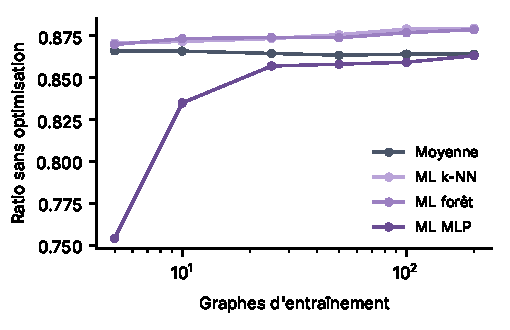
\includegraphics[width=0.6\linewidth]{fig_learning_curve.pdf}}
\caption{Ratio sans optimisation en fonction du nombre de graphes d'entraînement ($p=2$).}
\label{fig:lc}
\end{figure}

Avec seulement 5 graphes d'entraînement, le $k$-NN et la forêt aléatoire dépassent déjà la moyenne
($0{,}870$ contre $0{,}866$) ; ils progressent jusqu'à $0{,}879$ vers 100 graphes puis plafonnent
(figure~\ref{fig:lc}). Le réseau de neurones a besoin de beaucoup plus de données. Pour un usage réel,
quelques dizaines d'instances résolues suffisent.

\subsection{Généralisation à des graphes plus grands}

\begin{table}[h]
\centering
\small
\inclure{table_generalization.tex}{\input{\etude/table_generalization.tex}}
\caption{Modèles entraînés sur 6 à 10 sommets, testés sur 30 graphes de 12 sommets ($p=2$).}
\label{tab:gen}
\end{table}

Sur des graphes de 12 sommets, plus grands que tous ceux vus à l'entraînement, le classement est
inchangé (tableau~\ref{tab:gen}) : le $k$-NN propose des angles à 99,8\,\% du ratio final ($0{,}875$ contre
$0{,}877$). C'est le résultat le plus utile en pratique : on peut entraîner sur de petites instances,
simulables classiquement, puis initialiser le QAOA sur des instances que seul le matériel quantique
pourrait traiter.

% ----------------------------------------------------------------------------
\section{Discussion}

\paragraph{Pourquoi des modèles simples suffisent.}
Les angles optimaux dépendent surtout de quelques propriétés locales du graphe, en particulier des
degrés : les graphes réguliers d'un même degré partagent presque les mêmes angles~\cite{brandao2018}.
Un $k$-NN, qui retrouve les graphes déjà résolus les plus ressemblants, exploite directement cette
structure. Le réseau de neurones, plus flexible, manque de données pour l'apprendre.

\paragraph{Et le classique ?}
Sur ces instances, la recherche locale classique trouve la coupe exacte en $0{,}6$\,ms en moyenne, et
la force brute en $0{,}1$\,ms ; le QAOA à $p=3$ n'atteint qu'un ratio moyen de $0{,}93$. Ce travail
n'établit donc aucun avantage quantique. Il montre qu'une partie du coût classique du QAOA -- la boucle
d'optimisation -- peut être fortement réduite par apprentissage, ce qui compte sur un matériel où chaque
évaluation se paie en temps de calcul réel.

\paragraph{Limites.}
Simulation exacte sans bruit ; graphes non pondérés et de petite taille ; caractéristiques choisies à la
main ; nombre d'évaluations mesuré avec des gradients par différences finies, alors que le matériel
utiliserait la règle du \emph{parameter shift} et des estimations bruitées.

\paragraph{Perspectives.}
Graphes pondérés ; réseaux de neurones sur graphes (GNN) à la place des caractéristiques manuelles ;
effet du nombre fini de mesures ; démarrage à chaud par relaxation classique~\cite{egger2021} ;
exécution sur un processeur IBM Quantum.

% ----------------------------------------------------------------------------
\section{Conclusion}

Prédire les angles du QAOA à partir de la structure du graphe est simple et efficace : un modèle des
$k$ plus proches voisins entraîné sur quelques dizaines de graphes propose des angles à 99\,\% de
l'optimum, réduit de 44\,\% le nombre d'évaluations du circuit par rapport à la meilleure heuristique
sans apprentissage, et généralise à des graphes plus grands. L'apprentissage automatique ne remplace
pas le calcul quantique, mais il en réduit le coût classique d'accompagnement.

% ----------------------------------------------------------------------------
\begin{thebibliography}{9}

\bibitem{farhi2014}
E.~Farhi, J.~Goldstone et S.~Gutmann.
\newblock A quantum approximate optimization algorithm.
\newblock arXiv:1411.4028, 2014.

\bibitem{zhou2020}
L.~Zhou, S.-T. Wang, S.~Choi, H.~Pichler et M.~D. Lukin.
\newblock Quantum approximate optimization algorithm: performance, mechanism, and implementation on
near-term devices.
\newblock \emph{Physical Review X}, 10:021067, 2020.

\bibitem{brandao2018}
F.~G.~S.~L. Brandão, M.~Broughton, E.~Farhi, S.~Gutmann et H.~Neven.
\newblock For fixed control parameters the quantum approximate optimization algorithm's objective
function value concentrates for typical instances.
\newblock arXiv:1812.04170, 2018.

\bibitem{khairy2020}
S.~Khairy, R.~Shaydulin, L.~Cincio, Y.~Alexeev et P.~Balaprakash.
\newblock Learning to optimize variational quantum circuits to solve combinatorial problems.
\newblock \emph{Proceedings of the AAAI Conference on Artificial Intelligence}, vol.~34, 2020.

\bibitem{egger2021}
D.~J. Egger, J.~Mareček et S.~Woerner.
\newblock Warm-starting quantum optimization.
\newblock \emph{Quantum}, 5:479, 2021.

\bibitem{goemans1995}
M.~X. Goemans et D.~P. Williamson.
\newblock Improved approximation algorithms for maximum cut and satisfiability problems using
semidefinite programming.
\newblock \emph{Journal of the ACM}, 42(6):1115--1145, 1995.

\bibitem{pennylane}
V.~Bergholm \emph{et al.}
\newblock PennyLane: Automatic differentiation of hybrid quantum-classical computations.
\newblock arXiv:1811.04968, 2018.

\end{thebibliography}

\end{document}
